\chapter{Results}
\index{Results@\emph{Results}}%
\section{Introduction to Results}
To validate the models outlined as more than just a theoretical exercise in modeling, we engineer test cases based on standard IEEE power grids. We choose to use the 30 bus and 57 bus systems in order to capture effects on a large enough scale to demonstrate the model's applications. We hope this can extend into practical uses later on while the tests remain small enough that model run time stays reasonable. To convert these from standard test grids to DC versions for use in this model, reactive/imaginary power flow is dropped leaving only real power flow.

We assume also that the resulting road network for the area corresponding to the power network's service area can be represented with a Watts-Strogatz network, which is a network that connects each node of a graph to the $k$ nearest neighbors and then has probability $p$ of connecting any two nodes chosen. These networks exhibit the ``small world" property where any two arbitrarily distant nodes can be connected using only a small number of edges. Based on the literature on statistical analyses of road network topologies \cite{LammerEA2006} \cite{ChanEA2011} this is a serviceable but imperfect assumption to model  a semi-abstracted road grid. Ideally the real topology of a hurricane struck area should be used, but for a computational and modeling effort to draw insight into joint repair efforts, the contrived Watts-Strogatz based network suffices as it avoids having a full road model that would dramatically complicate the routing parts of the modeling by including dummy nodes in the routing efforts of every major intersection.

We then overlay a Watts-Strogatz graph with connection to the 3 nearest neighbor nodes and .03 global connectivity (i.e each node has a 3\% chance of being connected to any other node) as mentioned earlier based on fitting power buses to a grid. The key reason for fitting based on a grid is to maintain triangle inequalities. Random edge length generation is not guaranteed to follow triangle inequalities when computing distances. Having a network that violates triangle inequalities (Distance from A to B + distance from B to C is greater than or equal to distance from A to C) is both unrealistic to ``real world" situation as well as altering the solutions of routing problems \cite{FlemingEA2013}. We plan this so that travel time between opposite sides of the network are about 3 hours so that routing times are not trivial compared to repair times. We arbitrarily define repair times to be 5 hours for damaged nodes representing replacement of easy to fix components like breakers and downed lines inside the substation. More severe damage resulting from flooding and/or corrosion can take months to repair and is therefore outside the scope of immediate post-disaster response. We assume lines have a repair time of 1 hour plus a variable amount based on the geographical length of the line from our grid fit. We let the length of a shift be 12 hours to update the status of the grid twice per day. We acknowledge these times are somewhat arbitrary, but without loss of generality, data from a power utility can be fed in, so these arbitrary repair times suffice to warrant the utility of the underlying model.

To show validity, we first solve out a base damage instance for both grid topologies, then conduct perturbations of respectively weather damage, road topology, damage intensity, and power grid topology. We do this to show that the model is valid for a large variety of inputs and therefore can be presumed to be valid when applied to real world hurricane and network data. It is worth noting that not every model solves the repair horizon all the way to nominal operation. We cut off the computing at the same number of shifts per power grid topology so that everything plans to the same repair horizon to make comparison across instances valid.

\section{Nominal Operation}
To provide a point of comparison for damage and repair modeling, we look first at the case of nominal operation. Figure 3.1 shows the layout of the IEEE 30 bus network that has been overlaid with a road network as outlined above. The grid has a total demand of $283$ MW as modeled. The network has node 4 being the site of largest demand and node 0 being the site with the most generation capacity.
\begin{figure}[htbp]
	\centering
	
	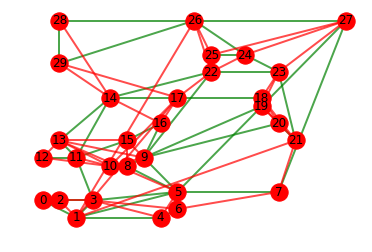
\includegraphics[width=.9\linewidth]{GridLayout.png}
	\caption{Overlaid power grid in green with road network in red}
	\label{fig:sub1}

\end{figure}

We also use the IEEE 57 test network, which has significantly more demand as it is loosely based on a representation of the American Midwest power grid in the 1960s. This test case from IEEE allows us to validate a larger network that has proportionally more demand and more complexity. 

\section{Geographically Clustered Damage}
Looking at our first case to validate the model, we manually apply geographically clustered damage to both road and power network. The damage in this case is concentrated where several damaged elements are next to each other in varying locations around the power grid. We show this in Figure 3.2 with damaged elements in red and operational elements in green. Of note here is that damaged substations have a damaged line close by.


\begin{figure}[htbp]
	\centering
	
	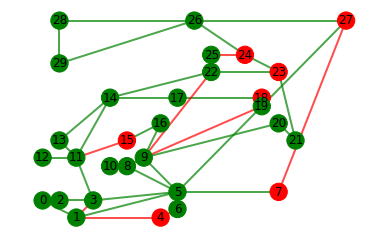
\includegraphics[width=.9\linewidth]{BaseCaseDamagePlot.png}
	\caption{IEEE 30 bus network with the base case damage applied and shown as red elements}
	\label{fig:sub1}
\end{figure}

For the base case on the 30 bus network, damage is applied to approximately one third of road segments, one quarter of power buses, and one third of power lines based on the damage modeling from the literature review. The following repair curves are generated from the model as stated earlier. This instance as well as all following instances are solved to a 1\% optimality gap. The reason for this is based on running instances, the final solution was found before this point.  

\begin{figure}[htbp]
	\centering
	
	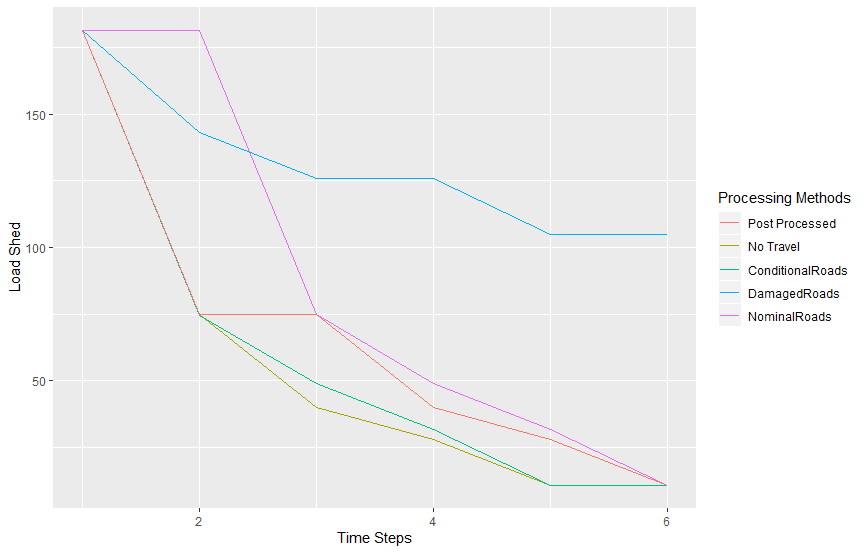
\includegraphics[width=.9\linewidth]{Rplot37.png}
	\caption{Load shed by shift in the 30 bus base instance}
	\label{fig:sub1}
\end{figure}
\begin{table}[htbp]
	\centering
	\caption{Total load shed over the repair horizon for the base instance}
	\resizebox{\columnwidth}{!}{\begin{tabular}{|c|c|c|c|c|}
	\hline	
	 Road First & Power First & Uncoordinated Repairs  &Post Processed & Lower Bound \\\hline
		291.7 & 479.4 & 291.7& 367.8 & 247.1 \\	
		\hline
	\end{tabular}}
	
	\label{time}
\end{table}
We conclude from Figure 3.3 as well as Table 3.1's summary of total unsatisfied demand across the repair horizon that changes in processing and interaction between models has meaningful impact on outcomes. It is worth noting that between points at the start and end of each shift, the shape of the repair curve is unknown. We present it as linear for the sake of simple visualization. For this case, we find that solving the roads and then conditioning the power repairs on that road schedule yields the outcome closest to the lower bound. This method being better is predicated on the assumption that the road repair crews would need one full shift to get ahead of what roads are needed in the framework where the power utility is the priority decision maker. If that delay can be reduced, letting the power utility dictate the road repair schedule becomes the best schedule inside the context of minimizing unsatisfied power demand over the repair horizon.


\section{Varied Damage location}
Looking at our next case to validate the models, we apply randomly distributed damage to both road network and power grid of similar intensity to the base case.
\begin{figure}[htbp]
	\centering
	
	\centering
	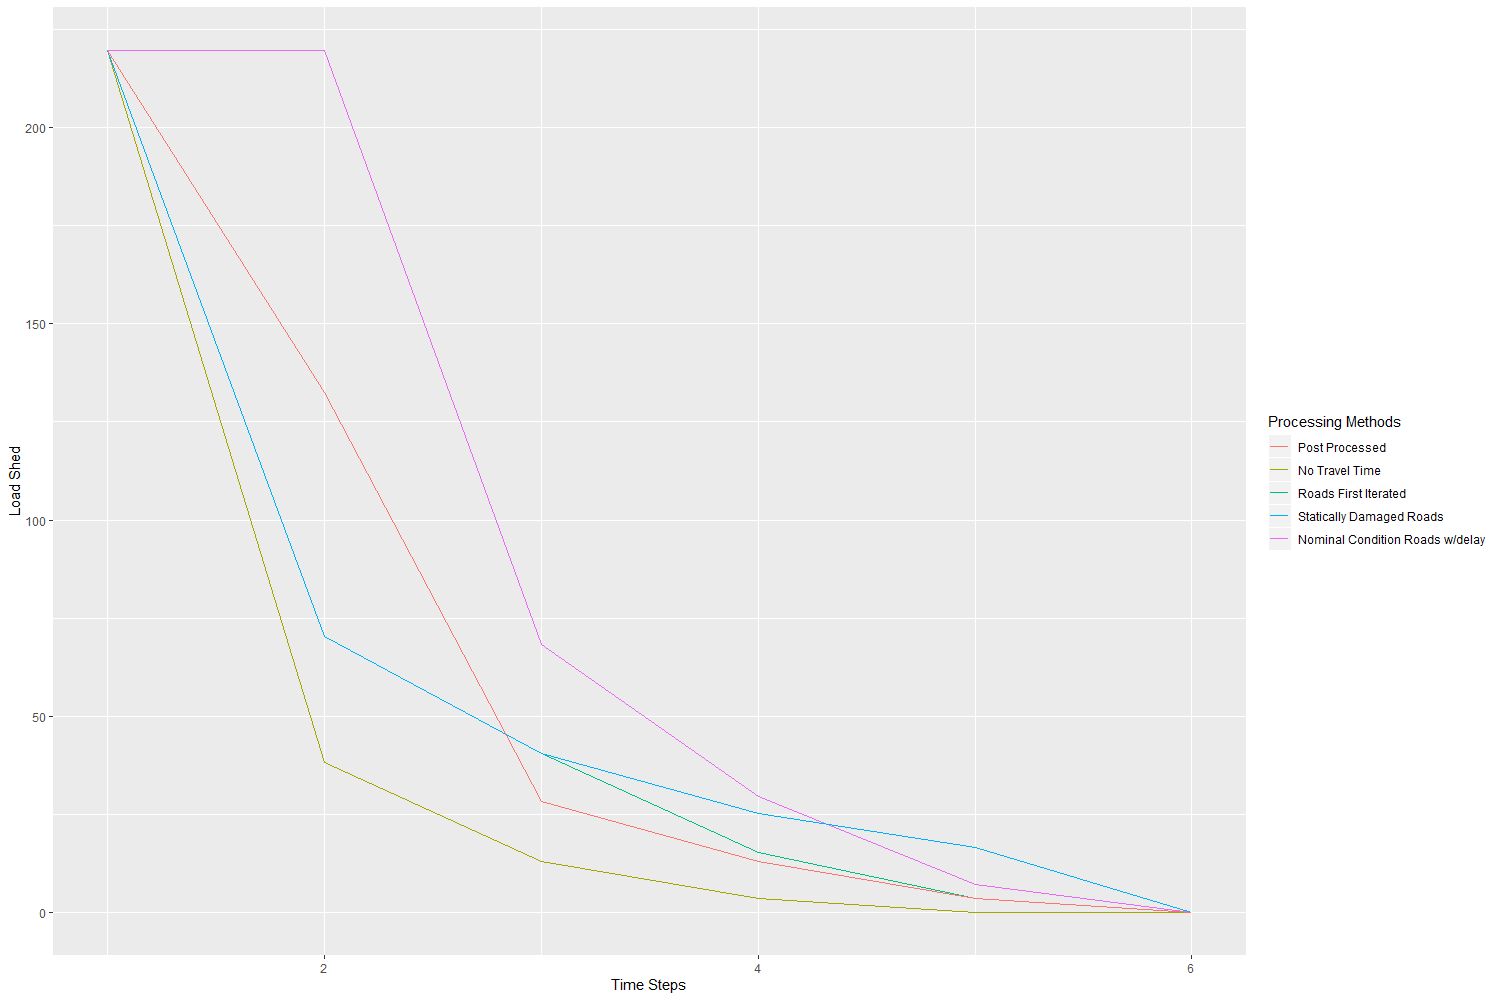
\includegraphics[width=.9\linewidth]{Rplot30Rand.png}
	\caption{Load shed by shift in the 30 bus randomized damage instance}
	\label{fig:sub1}
\end{figure}
\begin{table}[htbp]
	\centering
	\caption{Total load shed over the repair horizon for the random damage instance}
\resizebox{\columnwidth}{!}{\begin{tabular}{|c|c|c|c|c|}
		\hline	
		Road First & Power First & Uncoordinated Repairs  &Post Processed & Lower Bound \\\hline
		349.2 & 544.1 & 372.2 & 406.8 & 274.4\\	
		\hline
	\end{tabular}}
	
	\label{time}
\end{table}
We can draw comparable conclusions to the the geographically distributed base case, but for this instance as depicted in Figure 3.4 and Table 3.2. These repair curves having a rapid drop in load shed is due to the first several node and edge repairs being obvious choices. Given the rapid drop to baseline, the total lost load over the repair horizon is $544.8$ MW-shifts under the power first with delay framework as compared to the $349.2$ MW-shifts when solving the roads first or the $274.4$ MW-shifts of unsatisfied power demand in the lower bound solution. This is predicated on the delay to allow for road repairs to happen before they are needed for power grid repairs to occur with ideal transit times. Were this not to be the case, we find that the power first framework is the closest solution to the lower bound.

To demonstrate that the changes to how the road grid is treated drive much of the changes in satisfied power flow, we display the schedule for the random damage case in Table 3.3 for each of the interaction frameworks. The schedules are broadly similar in terms of what elements are prioritized, but by capturing the interactions with the road network, we can see that small perturbations to the schedule can dramatically change amount of demand unsatisfied over the repair horizon.

Of note is that not every element is repaired due to redundancies in the power grid, but that is justifiable in the context of disaster response as the first priority is satisfying demand and restoring redundant systems is a lower priority.  

\begin{table}[htbp]
	\centering
\caption{Repair schedule by interaction method for the 30 bus network with random damage}
	\begin{tabular}{|p{1.45cm}|p{2.1cm}|p{2.25cm}|p{2.5cm}|p{1.75cm}|p{1.75cm}|}
				
			\hline
			Shift Number & Road First & Power First & Uncoordinated Repairs  &Post Processed & Lower Bound \\\hline
			1 & Node 4, Line 2, Line 3 &Node 4, Line 2, Line 3, Line 17, Line 24& Node 4 and Line 3 & Node 7, Line 17, Line 3 & Node 4, Node 7, Line 3, Line 17 \\\hline
			2 & Node 7, Line 8, Line 35 & Node 7, Node 23& Node 7, Line 2, Line 24, Line 30,  & Node 4, Line 35&  Node 23, Node 24, Line 35\\\hline
			3 & Node 23, Node 24, Line 30 & Node 18, Node 24 & Node 15, Node 18, Line 17&  Node 23, Node 24 & Node 18, Line 2, Line 8, Line 20, Line 24, Line 30 \\\hline
			4 & Node 18, Line 14, Line 17, Line 24 & Node 20, Line 30, Line 35, Line 8, Line 14& Node 23, Line 8, Line 14, Line 35 & Node 18, Line 30, Line 2, Line 8, Line 20 & Node 15, Line 14\\\hline
			5 & Node 15, Line 20 & & Node 24 & Node 15, Line 24, Line 14&\\\hline
			6 & & & && \\\hline
	\end{tabular}
	
	\label{time}
\end{table}
\section{Varied Road Connectivity}
We now perturb the road topology of the network and solve a variation of the base case on the new road topology. The base-case road network was constructed as a Watts-Strogatz graph with neighbor connectivity 3 and global connectivity .03 as discussed earlier. To show the model as written is valid for multiple road topologies as well to show the impact of changing the road network, we permute the road network while keeping the power grid static. The new road topology is a different Watts-Strogatz graph with neighbor connectivity 2 and global connectivity .015. Additionally distances between nodes are increased by 25\%. This simulates the effect of the power grid in a more geographically spread out area with fewer direct paths between nodes.

The solutions are as follows in Figure 3.5 and 3.6 for first the unperturbed road network and then the perturbed road network. The damage here is another instance of random damage with a loss to 50\% of roads, 50\% of power lines, and 25\% of buses and substation in order to show the effects of a more severe hurricane and best the impact of the perturbed road network. 

\begin{figure}[htbp]
	\centering
	\includegraphics[width=.9\linewidth]{Rplot30unperturbed.png}
	\caption{Load shed by shift and method in a 30 bus instance before road perturbation}
	\label{fig:sub2}
	
	
\end{figure}
\begin{figure}[htbp]
	\centering
	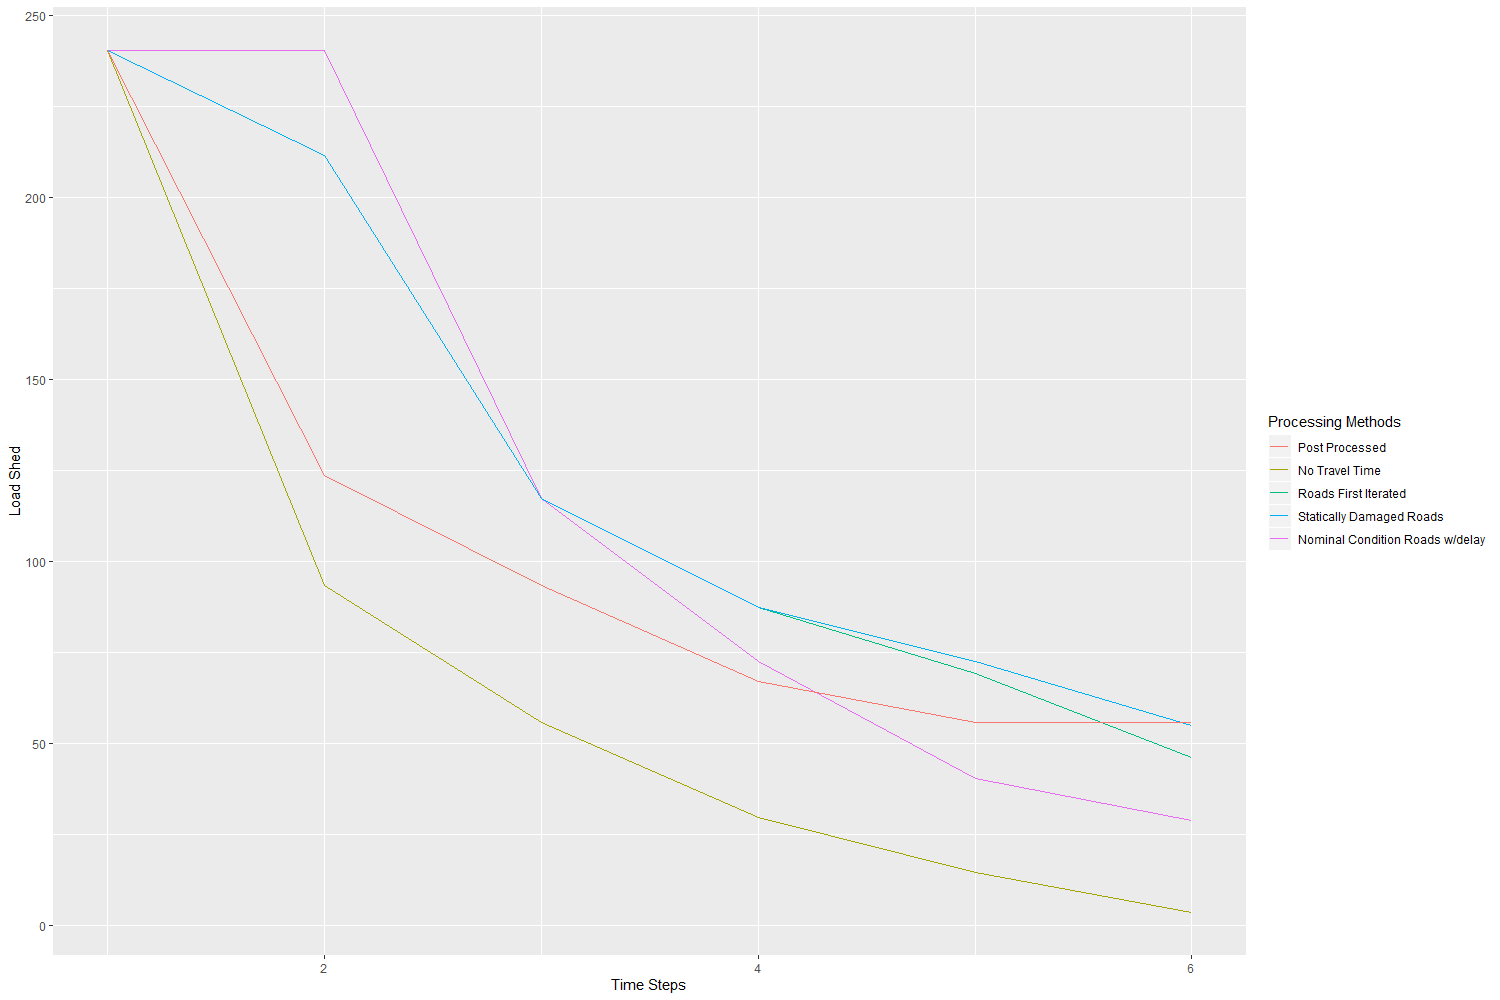
\includegraphics[width=.9\linewidth]{Rplot30Perturbed.png}
	\caption{Load shed by shift and method in a 30 bus instance for the geographically dispersed road network}
	\label{fig:sub2}
	
	
\end{figure}

We get largely intuitive changes here. Interaction frameworks that are on-face more sensitive to road changes (the uncoordinated repairs framework) have larger magnitudes of change in performance under perturbation of the road network. Figure 3.6 shows a markedly different curve set from Figure 3.5 where instead of a fairly steady decrease, we see a larger amount of damage carrying over into later parts of the repair horizon. Aditionally, there is far more deviation in framework solutions in the case where the roads are altered to be a more geographically distributed network. This is to be expected as more time within each shift is spent on the travel time causing fewer repairs to be done in each shift.

Of note here is that the heuristically solved version of the model without travel time and use of a post-processor performs much better (i.e closer to the lower bound) in the case with the road network perturbed to be more distant. This is  because the heuristic ignores road repair entirely in the name of not having to solve a mixed integer programming model. A version of the model where the road repair integer program is solved and used to generate time dependent road lengths for use in the post-processing heuristic would likely be significantly closer to the kind of solution the method would generate if deployed to real disaster response.

\section{Varied Damage Intensity}
We now perturb the base case for a higher damage instance in order to show model effectiveness for varying levels of damage. We show the higher damage in Figure 3.7
\begin{figure}[htbp]
	\centering
	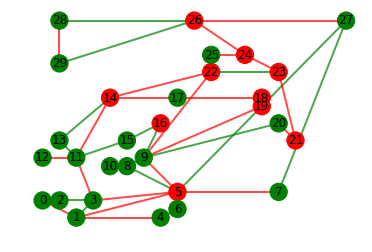
\includegraphics[width=.9\linewidth]{30BusSevereDamage.png}
	\caption{IEEE 30 bus network with the more severe damage applied and shown as red elements}
	\label{fig:sub2}
	
	
\end{figure}
\begin{figure}[htbp]
	\centering
	\includegraphics[width=.9\linewidth]{Rplot30scenario2.png}
	\caption{Load shed by shift in a 30 bus instance with increased damage}
	\label{fig:sub2}
	
	
\end{figure}
\begin{table}[htbp]
	\centering
	\caption{Total load shed over the repair horizon for the increased damage instance}
	\resizebox{\columnwidth}{!}{\begin{tabular}{|c|c|c|c|c|}
		\hline	
		Road First & Power First & Uncoordinated Repairs  &Post Processed & Lower Bound \\\hline
		447.9 & 548 & 454.2 & 477.7 & 327.9\\	
		\hline
	\end{tabular}}
	
	\label{time}
\end{table}

For larger amounts of damage on a network, the repair curve has a large initial drop followed by the similar amounts of tailing off seen in lower damage cases. This is because of most power grids having a few high priority node repair decisions for nodes that satisfy large amounts of the grid's demand. The remaining ~75MW of demand have less obvious decisions and depend more on the state of the road grid. This is seen clearly in Figure 3.8. While the post processed solution looks like it has a delay, but this is due to not fixing a particular node until the second shift and placing only line repairs in the first shift. We note here that uncoordinated repairs and solving the road repairs first generate the same repair curve. This is a consequence of the network having enough alternate routes that rerouting the repair crew does not alter the repair schedule. 
\section{Varied Grid Topology}
We now demonstrate the repair problem for a larger and more complex power grid in order to confirm model validity for larger scale problems. The road network is fit as it was for the base case where travel time from one side of the topology to the other is about 3 hours. We apply damage of comparable magnitude to the base case where damage is applied to approximately one third of road segments, one quarter of power buses, and one third of power lines
\begin{figure}[htbp]
	\centering
	\includegraphics[width=.9\linewidth]{Rplot57.png}
	\caption{Load shed by shift in the 57 bus instance}
	\label{fig:sub2}
	
	
\end{figure}

While the result for both solving the roads first and for solving with nominal condition roads with delay have similar behavior to previous cases' model interactions, the heuristic solution method of solving the lower bound and post-processing performs significantly worse. The reason for this is that a spatially larger power grid means that routing is a proportionally larger share of each shift, and ignoring that aspect until postprocessing results in solutions that get farther from the lower pound as the power grid grows spatially. In Figure 3.9, we see that both roads first and uncoordinated repairs framework have nearly the same load shed solution. This appears to be a flaw of how road damage is treated and suggests that a sparser road grid representation or higher proportion of road grid damage may be necessary to correctly capture the effects of road interactions for larger power grids.

\section{Model Runtimes}
Models are only useful if they can be implemented in a practical context. As disaster response planning is a somewhat time sensitive affair, a model that takes days or weeks to run is not useful as repairs need to start within the first few days. Based on using Gurobi 8.1.1 running on a i5-9600k CPU with 32gb of RAM running through the gurobipy interface for Python 3 for model building, model runtimes for road repairs range between 5 and 15 minutes on the 30 node case and 15-45 minutes on the 57 node case depending on the damage level. More damage leads to more possible decision options which means a longer runtime. Power repair model solution times range between 10-20 minutes for the IEEE 30 bus test network depending on interaction with the road network and 60-90 minutes for the IEEE 57 bus test network.


\section{Overall}
From the basket of demonstrated cases, we can see that interaction frameworks that allow more information sharing between road and power repairs are closer to the theoretical lower bound. As we make the assumption that power repairs that treat the road network as if it has been repaired to their needs requires a one shift delay in the start of repair operations, it is sub-par compared to solving the road network and then planning the power repairs based on that schedule. Were that assumption not to be valid, solving the power grid repairs under the presumption of nominal condition roads and then using those solutions to find a series of road repairs would be the best way of solving the repair problem if the only goal was to minimize total loss of satisfied demand in the power grid. Even with the delay, if the goal is to get the power grid back to nominal operation, solving the power first with the delay is better for higher damage cases. There are real reasons to give the road grid first-mover priority such as prioritizing flow in of humanitarian goods rather than restoration of power grid operations. Even under that interaction framework, power grid outcomes are better than they were under the schedule and post-process framework, suggesting that any coordination is still an improvement over methods that fail to capture the power/road interactions.


\section{Justifying the use of a Minimum Spanning Tree Approximation}

Now that we have presented several instances of the repair models, we can use these to go back and validate the use of our minimum spanning tree assumption when we first constructed the model.

In the above model we discuss the use of a minimum spanning tree to approximate the length of the route of a repair crew to reduce computational time. We demonstrate the validity of this by formulating the routing version of the problem, then running three instances to find first if we get the same (or at least a very similar) solution, and secondly to show the difference in runtime.

We begin by defining our sets and variables as above with the change that $Q_{ij}^t$ represents the inclusion of the shortest path from $i$ to $j$ in the tour at time $t$. We change $M^t$ from the length of the minimum spanning tree approximation of the route/tour length to the tour length itself. The routing model is then as follows:

\begin{equation}
\textnormal{Minimize}\sum_{i \in N} \sum_{t \in T} Y_{it}
\end{equation}
\textbf{subject to:}
\begin{eqnarray}
X_e^t = B_e (\theta_{o(e)}^t - \theta_{d(e)}^t), \hspace{5pt} \forall t \in T, \hspace{4pt} \forall e \in E\\
G_i^t - \sum_{e \in O(i)} X_e^t + \sum_{e \in D(i)} X_e^t = D_i-Y_i^t, \hspace{4pt} \forall t \in T, \hspace{4pt} \forall i \in N\\
0\leq G_k^t \leq P_{k} V_{k}^t, \hspace{4pt} \forall t \in T, \hspace{4pt} \forall k \in N\\
0\leq Y_i^t \leq D_i, \hspace{4pt} \forall t \in T, \hspace{4pt} \forall i \in N\\
-\overline{L_e}W_{e}^t \leq X_{e}^t \leq \overline{L_e}W_{e}^t, \hspace{4pt} \forall t \in T, \hspace{4pt} \forall e \in E\\
-\overline{L_e}V_{o(e)}^t \leq X_{e}^t \leq \overline{L_e}V_{o(e)}^t, \hspace{4pt} \forall t \in T, \hspace{4pt} \forall e \in E\\
-\overline{L_e}V_{d(e)}^t \leq X_{e}^t \leq \overline{L_e}V_{d(e)}^t, \hspace{4pt} \forall t \in T, \hspace{4pt} \forall e \in E\\
V_i^t \leq \sum_{t'=0}^{t-1} Z_i^{t'}+I_i, \hspace{4pt} \forall i \in N, \hspace{4pt} \forall t\in \{1,2,....t_{max}\}\\
W_{e}^t \leq \sum_{t'=0}^{t-1} U_{e}^{t'}+I_e, \hspace{4pt} \forall e \in E, \hspace{4pt} \forall t\in \{1,2,....t_{max}\}\\
M^t = \sum_{i \in N} \sum_{j \in N} {SP}_{ij}^t Q_{ij}^{t},  \hspace{4pt} \forall t \in T\\
\sum_{j \in N} Q_{ij}^t \geq Z_i^t, \hspace{4pt} \forall i \in N, \hspace{4pt} \forall t \in T\\
\sum_{j \in N} Q_{o(e)j}^t + \sum_{j \in N} Q_{d(e)j}^t \geq U_e^t, \hspace{4pt} \forall e \in E, \hspace{4pt} \forall t \in T\\
\sum_{j \in N} Q_{ij}^t - \sum_{j \in N} Q_{ji}^t = 0, \hspace{4pt} \forall i \in N, \hspace{4pt} \forall t \in T\\
\sum_{i,j \in S} Q_{ij}^t \leq |S|-1, \hspace{4pt} \forall S \subset N, \hspace{4pt} \forall t \in T\\
\sum_{e \in E} R_{e}U_e^t + \sum_{i \in N}R_{i}Z_i^t + M^t \leq F^t, \hspace{4pt} \forall t \in T\\
Q_{ij}^t,U_{e}^t,Z_{i}^t,W_{e}^t,V_{i}^t \in \{0,1\}. 
\end{eqnarray}

This model nearly the same as the model presented in Section 2.5, but the minimum spanning tree approximation to routing is replaced by a full routing problem in order to test the validity of the approximation we make. The changes are the replacement of constraints (2.31-2.33) in the original model with constraints (3.11-3.16). This more complex model generates the full route of the crew in terms of shortest paths between nodes rather than just determining what nodes they visit and providing a bound on what cost they pay to do so. 

We then solve a trio of instances check the validity of the minimum spanning tree assumption. Table 3.2 shows the optimum object function values and solution times of the corresponding models for the three instances. 
\begin{table}[htbp]
	\centering
	\caption{Runtime and objective values for minimum spanning tree and routing versions of the power repair problem}
	\resizebox{\columnwidth}{!}{\begin{tabular}{|c|c|c|c|c|}
			\cline{2-5}
			& \multicolumn{2}{c|}{MST} & \multicolumn{2}{c|}{Routing} \\
			\hline
			& MST Objective & MST Runtime & Routing Objective & Routing Runtime\\
			\hline
			Instance 1 (30 bus base instance)& $345.2$ & $25$ seconds   & $369.6$  & $639$ seconds  \\
			\hline
			Instance 2 (30 bus random damage instance) & $357.5$  & $15$ seconds & $406$ & $488$ seconds \\
			\hline
			Instance 3 (57 bus) & $2748$  & $4328$ seconds & no solution & $5400^*$ seconds\\
			
			\hline
	\end{tabular}}
	
	\label{time}
\end{table}

From this, we can see that the minimum spanning tree version of the model runs significantly faster and comes to a similar objective. The reason the 3rd instance has no solution for the routing based model is that these instances were run with a $90$ minute maximum runtime. At $90$ minutes, there was still a $22\%$ gap between the best incumbent solution and the lower bound solution in the branch-and-bound solver. While the second instance has a difference of 13.5\% between the objectives, the difference here is because of a single repair being moved to a later shift as a byproduct of the MST based model underestimating travel time. This leads us to believe this is an approximation that will be useful in planning disaster response. The step that would have to exist if the MST approximation is used is to solve the routing problem for the response crew between the selected elements. Determining the optimal route between less than 10 elements chosen for a shift by the MST based model is a simple and well solved problem.
